\documentclass[a4paper]{article}
\usepackage[left=1.7cm, right=1.7cm, top=2.5cm, bottom=2cm]{geometry} 
\usepackage{setspace}
%\renewcommand{\baselinestretch}{1.5} 
\usepackage{amsmath,amsthm,amssymb,scrextend}
\usepackage{fancyhdr}
\pagestyle{fancy}
\usepackage{lmodern}
\usepackage[british]{babel}
\usepackage[utf8]{inputenc}
\usepackage{graphicx}
\usepackage{hyperref}
\usepackage{titlesec}
\usepackage[backend=biber, style=apa]{biblatex}
\addbibresource{references.bib}
\usepackage{csquotes}
\usepackage{longtable}

\usepackage{lscape}


\titlespacing*{\section}
{0pt}{0pt}{15pt}
\titlespacing*{\subsection}
{0pt}{15pt}{5pt}
\titleformat{\section}[block]{\Large\bfseries\filcenter}{}{1em}{}

\pagenumbering{arabic}

\begin{document}

\lhead{Maximilian Kupi}
\chead{Master Thesis - Project Proposal}
\rhead{\today}

\textsl{}

\section*{The Adaption of Agile Methods and Principles in Public Administrations}
\begin{center}
%\subsection*{\hfill \hfill}
\end{center}

\noindent
\begin{spacing}{1.5}
%%%%%%%%%%%%%%%%%%%%%%%

\subsection*{Discussion of Academic Paper}
%1. Discuss one key academic paper that is the most relevant to your project. 
%You should summarise the paper,done 
%providing the title of the paper,done 
%the goal and achievement of the paper, done
%your criteria for selecting the paper, done
%solution proposed in the paper, done (?)
%data used in the paper, done
%methods used in the paper, done
%references to other (up to) 5 relevant papers.
The key academic paper for my project is the journal article \textit{"Agile Innovation Management in Government: A Research Agenda"} by Ines Mergel, Yiwei Gong, and John Bertot (\cite*{Mergel2018}). Its goal is to provide a (brief) overview of agile software development, analyse and synthesise existing literature on agility in government, and provide a series of future research questions. I have selected the paper since it is the most recent literature review on the substantive part of my topic, providing a comprehensive introduction into the research field.\par 
After motivating the need for agile governance based on the apparent change in citizens' expectations towards government services as well as the increased necessity to manage complex IT innovations (potentially involving AI, Big Data etc.), the authors state that agile government practices originate from the private sector software engineering domain and intend to "transform organizational culture and methods of collaboration to achieve higher level of adaptiveness” (\cite[p. 292]{Mergel2018}). In order to further illustrate the agile approach, the authors provide the \href{https://agilemanifesto.org/principles.html}{12 principles of agile software development} as laid down in the foundational work of the Agile Manifesto (\cite*{AgileManifesto2001}).\par 
Next, the authors explain their systematic literature review approach which they base on the PRISMA method developed by Moher et al. (\cite*{Moher2009}): Initially they searched the Web of Science and Google Scholar databases from 1988 to 2018 using the following pre-defined keywords: adapt* AND government, flex* AND government, agil* AND government. Getting over 100,000 hits, the authors then used an inclusion criteria-set to sort out the relevant articles, which ultimately left them with 33 articles for their analysis.\par 
Analysing the content of the respective papers, the authors find that the existing agile government studies are mainly empirical research and focus on the applications and practice of agile government approaches in various contexts. They identify the following four research streams:\par %
\begin{enumerate}
    \item \underline{Agile software development}: Focusing mainly on the particularities, benefits, and challenges of applying agile methods in IT related government projects, research from this stream finds that agile methods improve organisations' internal collaboration, communication, and speed. Moreover, agile approaches have been found to increase users' loyalty and satisfaction as well as the organizations' responsiveness to changing requirements in their environment. 
    \item \underline{Agile acquisition}: This research stream focuses on the necessary interplay of agile development approaches with new forms of acquisition and vendor management as well as the therewith connected difficulties. It finds that "agile contracting and acquisition practices help governments avoid vendor lock-in, and move away from proprietary applications and single-vendor contracts" (\cite[p. 296]{Mergel2018}). This in turn is said to enable governments to be more flexible, and better leverage the internal and external capacities. 
    \item \underline{Agile project management}: This stream focuses on applying agile methods in all aspects of government project management and assess the thereby involved drivers and barriers. It finds that agile methods improve governments ability to streamline projects and increase flexibility in delivery but tend to conflict with traditional leadership and management approaches in the public sector.
    \item \underline{Agile evaluation}: Finally, a largely underexplored research area is the evaluation of agile approaches. Here, researchers try to apply measurement and assessment methods from other areas like the private sector or engineering to measure agility and its impact in government. Authors find that through early validation and the evaluation of alternatives, agile methods tend to reduce costs and risks of public administration projects.
\end{enumerate}\par 
%
The authors of the paper summarize the findings from their literature review concerning gains and challenges in applying agile methods in the public sector as follows: "On the one hand, governments and the citizens whom they serve benefit from greater efficiencies, better designed and implemented applications, and cost savings. On the other hand, agile deployments require capacity, skills, culture, policy structures, and leadership that governments may not possess"(\cite[p. 298]{Mergel2018}).\par 
From these findings they derive possible future research questions like the following: What are the prerequisites for governments to engage in agile efforts, e.g., skills, capacity, policies, leadership? How can bureaucracies adapt or how can agile approaches be aligned with the needs of bureaucracies and their regulations? What is the required legal and regulatory environment to foster and promote agile efforts? How to measure and evaluate agility and its impact on government organizations? And finally, how do government structures and characteristics – centralized, size, engagement with public-private partnerships, innovation efforts, technology maturity, and others – impact the ability of governments to engage in agile methods?\par 
Further relevant references from the paper are:
\begin{itemize}
  \setlength\itemsep{0.01em}
    \item Torgeir Dingsøyr, Sridhar Nerur, Venugopal Balijepally, and Nils Brede Moe (\cite*{Dingsoyr2012}) "A decade of agile methodologies: Towards explaining agile software development"
    \item Yvonne Dittrich, Jan Pries-Heje, and Kristian Hjort-Madsen (\cite*{Dittrich2005}) "How to make government agile to cope with organizational change"
    \item Darrell K. Rigby, Jeff Sutherland, Hirotaka Takeuchi (\cite*{Rigby2016}) "Embracing agile"
    \item Janette Scott, Robyn Johnson, Michael McCullough (\cite*{Scott2008}) "Executing agile in a structured organization: Government"
\end{itemize}

%
\subsection*{Motivation}
%2. Motivation: why your project is interesting; describe the main goals of the project; what is the scientific question you are trying to answer; why you chose this goal
In today’s fast-paced world a high level of responsiveness and adaptability to changing user needs has become the key-skill of any organisation, be it private or public. Furthermore, citizens’ expectations of well-integrated and seamless government service experiences are constantly rising, with the bar being set higher and higher by extremely user-centred private sector companies every day. Lastly, the integration of advancements in digital and AI technologies demands for new, more flexible public governance structures. Hence, the adoption of agile methods in the public sector has become one of today’s mantras in public management practice and literature (\cite{Mergel2018, Vacari2015}). However, although the number of scholars investigating agile governance has constantly risen over the last years, academia still lacks a clear understanding of the concrete evolution and spread of agile methods in public administrations (\cite{Mergel2018}). In my master thesis I aim to help closing this research gap by answering the following research question: \textit{What is the evolution and spread of agile governance methods and principles in German, Austrian, and British public administrations?}
%
\subsection*{Task}
%§3. Task: what will you try to do in the thesis
In my thesis I will employ theory-informed, exploratory natural language processing based on web-scraped data to investigate the evolution and spread of agile methods in the German, Austrian and British government. In particular I will
\begin{enumerate}
  \setlength\itemsep{0.01em}
    \item identify websites of federal government ministries that mention relevant keywords related to agile methods (see \hyperref[Annex]{Annex});
    \item download the content and meta data of the respective websites;
    \item generate a corpus database of the crawled text data including the date of creation for each web-document;
    \item analyse the database with respect to the quantity and quality of the mentioned keywords and their context (word frequencies, topic models, sentiment analysis, word embeddings, context words etc.); 
    \item use the analysis results to generate an \textit{"Agile Methods Intensity Index"} and heat maps to compare the countries and/or ministries over time; and finally,
    \item draw conclusions based on the findings from the exploratory analysis in regard to similarities and differences between countries and/or ministries.
\end{enumerate}
%
%
\subsection*{Data}
%4. Data: what data will you use
To gather the data for my analysis I am setting up an own online data collection system to crawl and scrape data (specific agile governance related keywords and their context) from government websites.

%
\subsection*{Methods}
%5. Method: what method(s) you are planning to use
I plan to employ the following methods:
\begin{itemize}
  \setlength\itemsep{0.01em}
    \item Web-crawling / -scraping to get the data (R packages: Rcrawler, hrvest etc.)
    \item Natural language processing to construct the corpus and analyse topics, word representations, sentiments etc. (R packages: quanteda, spacyr, translateR, stm, text2vec, tidytext etc.)
\end{itemize}

%
\subsection*{Baseline}
%6. What baseline will you choose
I will focus on the analysis of German, Austrian and British ministries on the federal level, with Britain serving as a baseline. Potentially, I might extend my analysis to the federal state level.
\subsection*{Project Outcome}
%7. How would successful outcome of your project look like
This project will advance research by providing insights about the evolution and spread of agile method keywords on government websites. Furthermore, by creating an intensity index and heat maps over time it will allow an easy comparison between ministries and/or countries.
%
\begin{landscape}
\subsection*{Timeline}

%8. Timeline of the project, including a Gantt chart.
\hyperref[Gantt Chart]{Figure 1} illustrates the important tasks and deliverables over the project timeline.
\begin{figure}[h!]
	\centering
	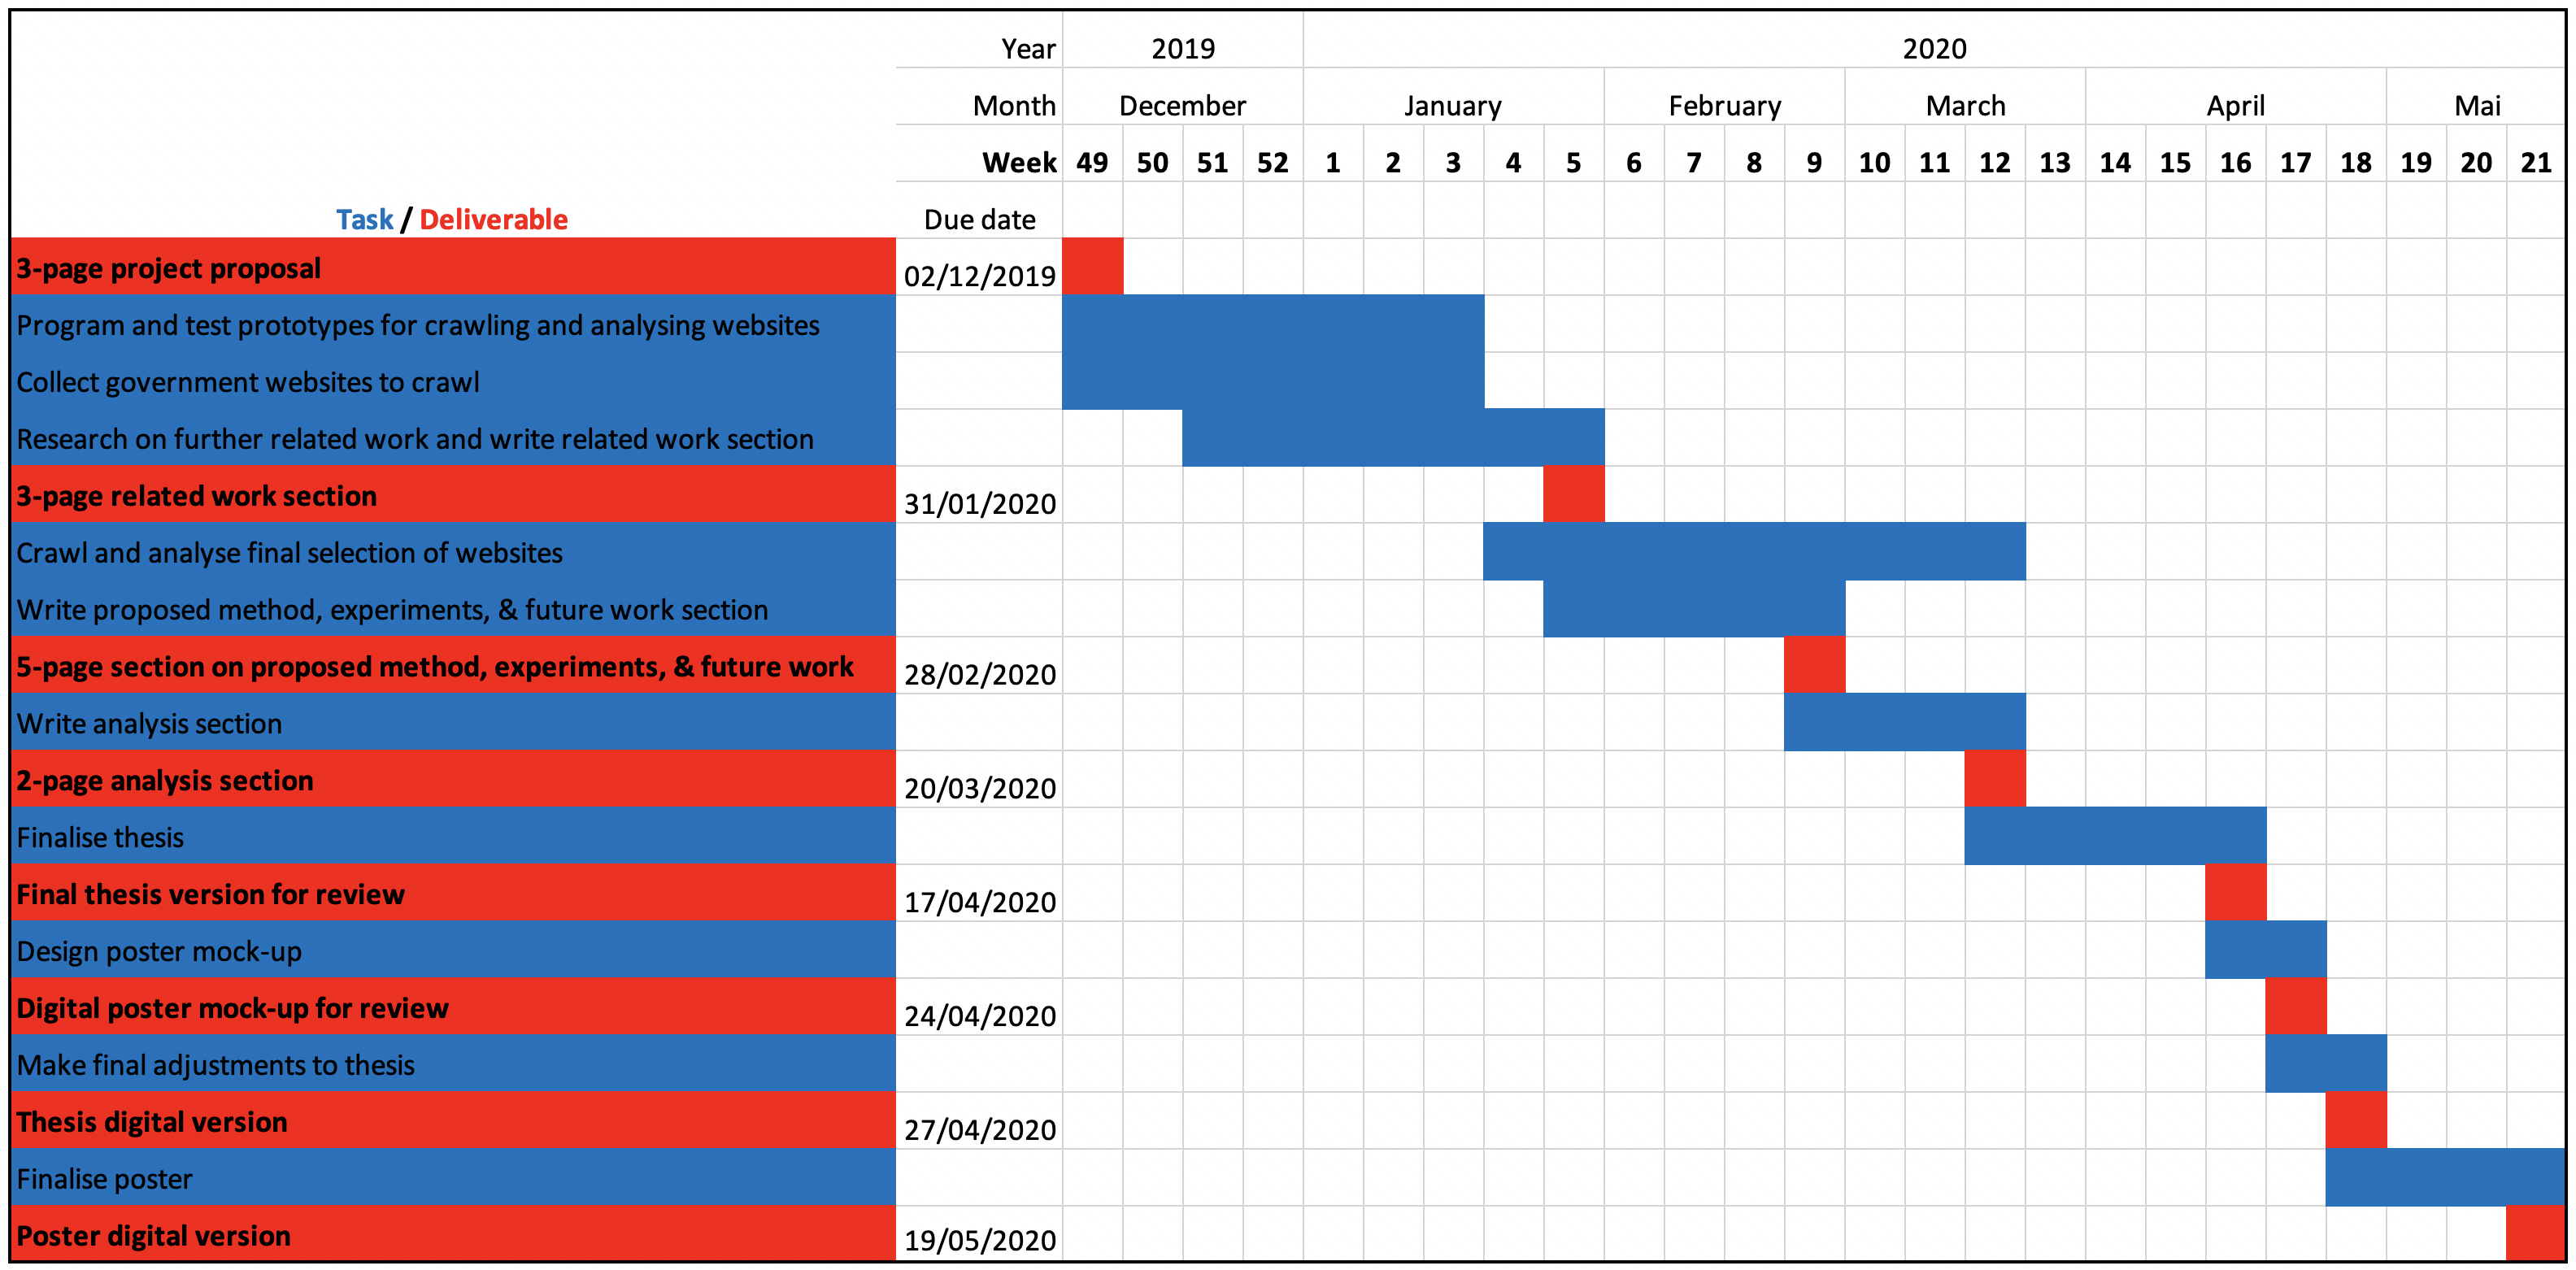
\includegraphics[height=.63\textwidth]{Latex/Gantt.png}
	\caption[Gantt chart depicting the project timeline]{Gantt chart depicting the project timeline}\label{Gantt Chart}
\end{figure}
\end{landscape}
%%%%%%%%%%%%%%%%%%%%%%%
\end{spacing}
\newpage
\printbibliography

\newpage
\pagenumbering{alph}
\begin{center}
\subsection*{\hfill Annex \hfill}\label{Annex}
\end{center}


\begin{longtable}{ p{5cm} p{5cm}}
	\caption{Search terms related to agile methods}\label{tab: search terms related to agile methods}\\
	%\renewcommand{\arraystretch}{1.4}
\hline
German & English\\
\hline
A-B-Tests	&	A-B testing\\
agile	&	agile\\
Agile Coach	&	agile coach\\
agile Entwicklung	&	agile development\\
agile Methoden	&	agile methods\\
agile Prinzipien	&	agile principles\\
agile Softwareentwicklung	&	agile software development\\
Agile Transition	&	agile transition\\
agile Werte	&	agile values\\
Agiles Manifest	&	Agile Manifesto\\
agiles Mindset	&	agile mindset\\
Agiles Projektmanagement	&	agile project management\\
Agilität	&	agility\\
Artefakt	&	artefact\\
Backlog	&	backlog\\
Bedürfnisse	&	needs\\
Benutzer	&	user\\
Brainstorming	&	brainstorming\\
bürgerzentriertes Design	&	citizen-centred design\\
Burndown Chart	&	burndown chart\\
Canvas	&	canvas\\
Co-Design	&	co-design\\
Co-Kreation	&	co-creation\\
Coach	&	coach\\
Community of Practice	&	community of practice\\
Continuous Delivery	&	continuous delivery\\
CoP	&	CoP\\
Cultural Probe	&	cultural probe\\
Daily Scrum	&	daily scrum\\
Definition of Done	&	definition of done\\
Definition of Ready	&	definition of ready\\
Design Challenge	&	design challenge\\
Design Thinking	&	design thinking\\
DoD	&	DoD\\
DoR	&	DoR\\
Einsichten	&	insights\\
Elevator Pitch	&	elevator pitch\\
Empathie	&	empathy\\
Empathy Maps	&	empathy maps\\
Entwicklungsteam	&	development team\\
Extremnutzer	&	usability\\
Extremnutzer Nutzer	&	extreme user\\
Facilitator	&	facilitator\\
fail fast	&	fail fast\\
fail forward	&	fail forward\\
Feature	&	feature\\
Feedback	&	feedback\\
Human Centred Design	&	human centred design\\
Ideation	&	ideation\\
Inkrement	&	increment\\
Iteration	&	iteration\\
Jobs-to-be-done	&	jobs-to-be-done\\
Kanban	&	kanban\\
Kanban-Board	&	kanban board\\
kollaboratives Design	&	collaborative design\\
Lean Startup	&	lean startup\\
Minimum Viable Product	&	minimum viable product\\
MVP	&	MVP\\
Nutzer	&	user\\
Nutzerbedürfnisse	&	user needs\\
Nutzererfahrung	&	user experience\\
Nutzerinterviews	&	user interviews\\
Nutzerreise	&	customer journey\\
Nutzerstory	&	user story\\
Nutzertest	&	user testing\\
nutzerzentriertes Design	&	user-centred design\\
Papierprototyp	&	paper prototype\\
Persona	&	persona\\
Pitch	&	pitch\\
Planning Poker	&	planning poker\\
Product Backlog	&	product backlog\\
Product Owner	&	product owner\\
Project Canvas	&	project canvas\\
Prototyp	&	prototype\\
Reframing	&	reframing\\
Release	&	release\\
Retrospektive	&	retrospective\\
Review	&	review\\
Rollenspiele	&	role-play\\
schlanke Softwareentwicklung	&	lean software development\\
Scrum	&	Scrum\\
Scrum Coach	&	Scrum coach\\
Scrum Master	&	Scrum master\\
Scrum Team	&	Scrum team\\
Service Design	&	service design\\
Sprint	&	sprint\\
Sprint Backlog	&	sprint backlog\\
Sprint Planning	&	sprint planning\\
Sprint Retrospective	&	sprint retrospective\\
Sprint Review	&	sprint review\\
Stakeholder Map	&	stakeholder map\\
Stand-up Meeting	&	stand-up meeting\\
Standpunkt	&	point of view\\
Story Map	&	story map\\
Storyboard	&	storyboard\\
Tagebuchstudien	&	diary study\\
Testen	&	testing\\
Timebox	&	time box\\
Timeboxing	&	timeboxing\\
visuelles Denken	&	visual thinking\\
Wicked Problem	&	wicked problem\\
Wireframe	&	wireframe\\
Workshop	&	workshop\\
		\hline
\end{longtable}
\end{document}